\documentclass[12pt,a4paper]{report}
\usepackage[utf8]{inputenc}
\usepackage{graphicx}
\usepackage{hyperref}
\usepackage{geometry}
\usepackage{longtable}
\usepackage{caption}
\usepackage{listings}
\usepackage{color}
\usepackage{xcolor}
\usepackage{amsmath}
\usepackage{booktabs}
\usepackage{float}
\usepackage{setspace}
\usepackage{array}
\usepackage{enumitem}
\usepackage{pgfplots}
\pgfplotsset{compat=1.18}

\geometry{left=30mm,right=25mm,top=25mm,bottom=25mm}
\onehalfspacing
\hypersetup{colorlinks=true, linkcolor=blue, citecolor=blue, urlcolor=blue}

\definecolor{codegreen}{rgb}{0,0.6,0}
\definecolor{codegray}{rgb}{0.5,0.5,0.5}
\definecolor{backcolor}{rgb}{0.97,0.97,0.97}
\lstdefinestyle{pythonstyle}{
    backgroundcolor=\color{backcolor},
    commentstyle=\color{codegreen},
    keywordstyle=\color{blue},
    numberstyle=\tiny\color{codegray},
    basicstyle=\ttfamily\footnotesize,
    breaklines=true,
    keepspaces=true,
    numbers=left,
    numbersep=5pt,
    language=Python,
    frame=single
}

\begin{document}

% -----------------------------------------
% IIIT Lucknow Thesis Title Page
% -----------------------------------------
\begin{titlepage}
    \centering

    \vspace*{1cm}

    % Title
    {\Large\bfseries A Data-Driven Framework for Wind Energy Deviation Penalty Optimization \par}

    \vspace{1.2cm}

    % Submission statement
    {\itshape A thesis submitted in partial fulfillment of the requirements for the award of the degree of \par}

    \vspace{0.6cm}

    % Degree
    {\large\bfseries MSc. \par}
    {\normalsize in \par}
    {\large\bfseries Data Science \par}

    \vspace{1cm}

    % By
    {\normalsize by \par}

    \vspace{0.5cm}

    % Candidate details
    {\large\bfseries Tapas Barman \par}
    {\normalsize\bfseries (Roll Number: MSD24021) \par}

    \vspace{1cm}

    % Supervision
    {\normalsize under the guidance of \par}

    \vspace{0.7cm}

    % Supervisors
    \begin{minipage}[t]{0.45\textwidth}
        \centering
        {\large\bfseries Dr. Sirsendu Sekhar Barman}\\
        {\normalsize Department of Mathematics}
    \end{minipage}%
    \hfill

    \vspace{1.2cm}

    % Logo
    \includegraphics[width=3.5cm]{iiitl.png}\par

    \vspace{0.5cm}

    % Institute name
    {\large\bfseries Indian Institute of Information Technology, Lucknow \par}
    {\normalsize\bfseries 2024-26 \par}

    \vspace{0.5cm}

    % Copyright
    {\small\textcopyright\ Indian Institute of Information Technology, Lucknow 2025. \par}

\end{titlepage}

% -----------------------------------------
% Certificate Page
% -----------------------------------------
\chapter*{CERTIFICATE}
\addcontentsline{toc}{chapter}{Certificate}

\vspace{1cm}

This is to certify that the thesis entitled \textbf{``A Data-Driven Framework for Wind Energy Deviation Penalty Optimization''} submitted by \textbf{Tapas Barman} who got his name registered on \textbf{Jul 2024} for the award of M.Sc degree at Indian Institute of Information Technology, Lucknow is absolutely based upon his own work under the supervision of \textbf{Dr. Sirsendu Sekhar Barman}, Department of Mathematics, Indian Institute of Information Technology, Lucknow - 226 002, U.P., India and that neither this thesis nor any part of it has been submitted for any degree or any other academic award anywhere before.

\vspace{4cm}

\begin{minipage}[t]{0.48\textwidth}
    Dr. Sirsendu Sekhar Barman\\
    Department of Mathematics\\
    Indian Institute of Information Technology\\
    Pin - 226002, INDIA
\end{minipage}
\hfill
\begin{minipage}[t]{0.48\textwidth}
    \raggedleft
    \rule{6cm}{0.4pt}\\
    Supervisor Signature
\end{minipage}

\vspace{2cm}

% -----------------------------------------
% Authorship Page
% -----------------------------------------
\chapter*{AUTHORSHIP}
\addcontentsline{toc}{chapter}{Authorship}

\vspace{1cm}

I, \textbf{Tapas Barman}, declare that this thesis titled, \textbf{``A Data-Driven Framework for Wind Energy Deviation Penalty Optimization''} and the work presented in it are my own. I confirm that:

\begin{itemize}
    \item This work was completed entirely while in candidature for Master of Science degree at Indian Institute of Information Technology, Lucknow.

    \item Where I have consulted the published work of others, it is always cited.

    \item Wherever I have cited the work of others, the source is always indicated. Except for the aforementioned quotations, this thesis is solely my work.

    \item I have acknowledged all major sources of information.
\end{itemize}

\vspace{2cm}

\noindent\textbf{Signature:} \\[1ex]
\includegraphics[width=5cm]{sig.jpeg} \\[2ex]

\noindent\textbf{Date: 08-03-2026}

% -----------------------------------------
% Acknowledgements Page
% -----------------------------------------
\chapter*{Acknowledgements}
\addcontentsline{toc}{chapter}{Acknowledgements}

\vspace{1cm}

I would like to express my sincere gratitude to my supervisor, \textbf{Dr. Sirsendu Sekhar Barman}, whose guidance, expertise, and continuous encouragement were instrumental throughout the execution of this project. I extend my thanks to all faculty members of the MSc Data Science programme for providing a strong academic foundation. I am also grateful to the Southern Regional Power Committee (SRPC) for maintaining publicly accessible Grid DSM data, and to the open-source communities behind Python, XGBoost, and windpowerlib, whose tools made this work possible.

\vfill

\noindent
\begin{minipage}[t]{0.48\textwidth}
    Lucknow\\
    March 2026
\end{minipage}
\hfill
\begin{minipage}[t]{0.48\textwidth}
    \raggedleft
    Tapas Barman
\end{minipage}

% -----------------------------------------
% Abstract
% -----------------------------------------
\chapter*{ABSTRACT}
\addcontentsline{toc}{chapter}{Abstract}

Wind energy is growing rapidly across India, but its unpredictable nature creates a major financial problem. India's power regulator (CERC) requires wind farms to declare how much electricity they will produce in 96 time-slots of 15 minutes each, every day in advance. If the actual generation differs from this declaration by more than 10\%, the wind farm is financially penalised. These penalties, known as Deviation Settlement Mechanism (DSM) charges, can cost a single wind plant several Crores of Rupees per year.

This project builds a smart forecasting system that significantly reduces these penalties. It works in two stages: first, it uses the laws of physics (specifically how wind speed, air temperature, and pressure affect power output) to generate a theoretical power forecast. Second, it uses a machine learning model (XGBoost) trained on 10 months of real historical data from the RSOPL Koppal 75 MW wind plant in Karnataka to correct the remaining errors that physics alone cannot capture.

The research uses real official data from the Southern Regional Power Committee (SRPC) covering 29,568 fifteen-minute blocks between April 2025 and February 2026. Early results show that the baseline penalty from the SRPC data stood at \textbf{Rs.\ 41.34 Crores}. The expected impact of the full model is to reduce this significantly through more accurate scheduling.

\vspace{0.5em}
\noindent\textbf{Keywords:} Wind Power Forecasting, CERC DSM, Physics-Informed ML, XGBoost, 96-Block Schedule, SRPC, India.

\tableofcontents
\listoftables

% -----------------------------------------
\chapter{Introduction}

\section{Background}

India is building one of the world's largest renewable energy systems, with a target of 500 GW of clean power by 2030. Wind energy is a major pillar of this plan, especially in southern states like Karnataka, Tamil Nadu, and Andhra Pradesh, which together host thousands of wind turbines.

Unlike a coal or gas plant that generates power on demand, a wind farm produces electricity only when the wind blows. This unpredictability is the root cause of the problem this project addresses.

\section{The Grid Scheduling Problem}

India's power grid must be kept in perfect balance at all times. The Indian Electricity Grid Code (IEGC) requires every wind farm to submit a generation schedule 1.5 to 2 hours in advance, broken into \textbf{96 time blocks of 15 minutes each} for the coming day. This is called the \textit{day-ahead schedule}.

If the wind farm then produces significantly more or less electricity than it declared, the Central Electricity Regulatory Commission (CERC) applies financial penalties under the \textbf{Deviation Settlement Mechanism (DSM)}. These penalties increase sharply depending on how large the error is.

\section{The Financial Impact}

This research analysed 10 months of official government data for the ReNew Surya Ojas Private Limited (RSOPL) wind plant in Koppal, Karnataka. The data revealed that this single plant accumulated approximately \textbf{Rs.\ 41.34 Crores} in under-injection (under-production) penalties in just 10 months.

This massive financial loss is caused by one main issue: existing forecasting models are simply not accurate enough at the 15-minute block level. They are designed for large geographic regions and miss the local wind behaviour that happens at a specific wind farm site.

\section{The Proposed Solution}

This project proposes a two-stage forecasting system called the \textbf{Physics-Informed Predictive Machine Learning (PI-PML)} pipeline:

\begin{enumerate}
    \item \textbf{Stage 1 — Physics Baseline:} The first stage uses well-established physics equations to calculate how much power the wind turbines should theoretically generate, based on weather forecast data (wind speed, temperature, and air pressure).
    \item \textbf{Stage 2 — Machine Learning Correction:} The second stage uses an XGBoost machine learning model to detect and fix the systematic errors that the physics calculation still makes. This model was trained using 10 months of real historical generation records from the RSOPL plant.
\end{enumerate}

The final output is a corrected 96-block day-ahead generation schedule that is significantly more accurate than the existing industry standard.

\section{Research Objectives}

\begin{enumerate}
    \item To collect and process 10 months of official SRPC 15-minute generation data for use as machine learning training labels.
    \item To build a Physics Engine that converts weather forecast data into theoretical power estimates using atmospheric science equations.
    \item To train an XGBoost model on the gap between the physics estimate and real generation, so it can predict and correct future errors.
    \item To simulate and quantify the financial savings achieved by the improved schedule using CERC's official penalty rules.
    \item To explore probabilistic forecasting (Low/Medium/High confidence ranges) to help the plant operator choose a financially safer schedule submission.
\end{enumerate}

\section{Current Progress Overview}

\begin{table}[H]
    \centering
    \caption{Project Phase Completion Status}
    \begin{tabular}{p{6.5cm}cc}
        \toprule
        \textbf{Phase} & \textbf{Status} & \textbf{Chapter} \\
        \midrule
        Regulatory Research (CERC DSM) & \textcolor{green}{\textbf{Complete}} & 2 \\
        Case Study: RSOPL Koppal Plant & \textcolor{green}{\textbf{Complete}} & 2 \\
        Baseline Financial Audit (Rs.\ 41.34 Cr) & \textcolor{green}{\textbf{Complete}} & 2 \\
        SRPC Data Collection \& Pipeline & \textcolor{green}{\textbf{Complete}} & 3 \\
        NWP Data Source Evaluation & \textcolor{green}{\textbf{Complete}} & 3 \\
        Physics Engine (Weather to Power) & \textcolor{green}{\textbf{Complete}} & 4 \\
        XGBoost Residual Model Training & \textcolor{orange}{\textbf{In Progress}} & 5 \\
        Probabilistic Confidence Intervals & \textcolor{red}{\textbf{Planned}} & 5 \\
        Financial Optimisation \& Validation & \textcolor{red}{\textbf{Planned}} & 5 \\
        \bottomrule
    \end{tabular}
\end{table}

% -----------------------------------------
\chapter{Research Foundations and Problem Validation}

\section{How CERC DSM Penalties Work}

\subsection{The Basic Mechanism}

Every wind farm in India must submit a day-ahead schedule showing how much electricity it expects to generate for each of the 96 fifteen-minute slots in the coming day. Once submitted, the farm is expected to deliver that exact amount.

When the actual generation differs from the declared amount, CERC calculates a financial penalty or rebate. This system is called the \textbf{Deviation Settlement Mechanism (DSM)}.

\subsection{The 10\% Tolerance Band}

CERC allows a small tolerance for small errors (up to 10\% of the plant's maximum capacity). Beyond this, penalties kick in and get progressively more expensive:

\begin{table}[H]
    \centering
    \caption{CERC DSM 2024 Penalty Band Structure}
    \begin{tabular}{cll}
        \toprule
        \textbf{Band} & \textbf{Error Size (of max capacity)} & \textbf{Penalty} \\
        \midrule
        1 & 0\% to 10\% & No penalty (safe zone) \\
        2 & 10\% to 20\% & 10\% of the current electricity price \\
        3 & 20\% to 30\% & 20\% of the current electricity price \\
        4 & More than 30\% & 30\% of the current electricity price \\
        \bottomrule
    \end{tabular}
\end{table}

\textbf{Evening hour trap:} Between 6 PM and 10 PM, electricity demand peaks as solar generation drops. During this window, the penalty price is 2.5 times higher than normal. Mis-forecasting during these hours is extremely expensive.

\textbf{Example:} For a 75 MW plant, the 10\% threshold means just 7.5 MW of error triggers penalties. A wind gust pushing output 8 MW above the declared schedule is enough to enter Band 2 and start accumulating charges across multiple consecutive blocks.

\section{Case Study: RSOPL Koppal Wind Farm}

\subsection{Why This Plant Was Chosen}

The ReNew Surya Ojas Private Limited (RSOPL) wind cluster in Koppal, Karnataka was selected for this study because:
\begin{itemize}
    \item Its official 15-minute generation data is publicly available from the SRPC government portal.
    \item The Koppal region has highly variable wind conditions due to its hilly terrain, making it a challenging and realistic test case.
    \item CERC legal petition records confirm this plant has been repeatedly penalised under DSM, providing real-world validation of the problem.
\end{itemize}

\subsection{Plant Details}

\begin{table}[H]
    \centering
    \caption{RSOPL Koppal Wind Farm --- Key Specifications}
    \begin{tabular}{ll}
        \toprule
        \textbf{Detail} & \textbf{Value} \\
        \midrule
        Location & Koppal District, Karnataka, India \\
        GPS Coordinates & 15.34\textdegree N, 76.15\textdegree E \\
        Registered Capacity & 75 MW \\
        Turbine Type & Vestas class (3 MW per turbine) \\
        Hub Height & 100 metres \\
        Rotor Blade Span & 112 metres diameter \\
        Power Onset Wind Speed & Approx.\ 3 m/s (cut-in) \\
        Full Rated Wind Speed & Approx.\ 12 m/s \\
        Safety Shutdown Speed & Approx.\ 25 m/s (cut-out) \\
        Grid Operator & SRLDC (Southern Regional Load Despatch Centre) \\
        Data Source & SRPC Public DSM Archives \\
        \bottomrule
    \end{tabular}
\end{table}

\section{Baseline Financial Audit}

To prove why this project is necessary, a financial audit of 10 months of official SRPC data was performed. The results are summarised below:

\begin{table}[H]
    \centering
    \caption{Financial Audit of RSOPL Koppal --- April 2025 to February 2026}
    \begin{tabular}{lr}
        \toprule
        \textbf{Metric} & \textbf{Amount (Rs.)} \\
        \midrule
        Cumulative Under-production Penalties & Rs.\ 41,34,83,388 \\
        Cumulative Over-production Charges & Rs.\ 31,30,81,483 \\
        \midrule
        \textbf{Net Financial Liability (Under-production)} & \textbf{Rs.\ 41.34 Crores} \\
        \bottomrule
    \end{tabular}
\end{table}

\textbf{Key finding:} The plant occasionally produces more than scheduled (and gets some credit for that), but the dominant problem is \textbf{under-production}: the wind drops unexpectedly and the plant fails to deliver its declared schedule. Under-production during evening peak hours hits the 2.5$\times$ pricing multiplier and causes the majority of the penalty liability. This Rs.\ 41.34 Crore figure is the benchmark the PI-PML model must beat.

% -----------------------------------------
\chapter{Data Engineering}

\section{Two Data Sources, Two Different Jobs}

The pipeline uses two completely different data sources, each with a distinct role:

\begin{table}[H]
    \centering
    \caption{Summary of Data Sources and Their Roles}
    \begin{tabular}{p{3.5cm}p{4.5cm}p{4.5cm}}
        \toprule
        & \textbf{SRPC Historical Data} & \textbf{NWP Weather Forecast} \\
        \midrule
        \textbf{What it is} & Official 15-min generation records from the government & Future weather forecast from a global model \\
        \textbf{Role in pipeline} & Training labels for XGBoost & Live input to the Physics Engine \\
        \textbf{When used} & Once (offline), to build the model & Every day, to run forecasts \\
        \textbf{Source} & SRPC public portal & NOAA GFS servers \\
        \bottomrule
    \end{tabular}
\end{table}

\textbf{The key distinction:} SRPC data teaches the model what errors look like in the past. Weather forecast data tells the model what is likely to happen tomorrow. These are never mixed during live operation.

\section{Weather Forecast Systems Compared}

Before choosing which weather data source to use for live forecasting, three major systems were evaluated:

\begin{table}[H]
    \centering
    \caption{Comparative Analysis of Candidate NWP Weather Systems}
    \begin{tabular}{p{3.8cm}p{2.8cm}p{2.8cm}p{3.2cm}}
        \toprule
        \textbf{Feature} & \textbf{NASA GEOS FP} & \textbf{NOAA GFS} & \textbf{Bharat Forecast System (BFS)} \\
        \midrule
        Run by & NASA (USA) & NOAA (USA) & IITM / NCMRWF (India) \\
        Wind Height Data & 50 m & 100 m & 120 m \\
        Grid Size & $\sim$25 km & $\sim$28 km & \textbf{6 km (Best)} \\
        Update Frequency & Every 12 hrs & \textbf{Every 6 hrs} & Every 12 hrs \\
        Ease of Access & Easy (URL) & \textbf{Easiest (API)} & Difficult (Registration) \\
        India-specific tuning & No & No & \textbf{Yes (Monsoon tuned)} \\
        \bottomrule
    \end{tabular}
\end{table}

\textbf{Decision: NOAA GFS was chosen} as the primary system for the following reasons:
\begin{itemize}
    \item It directly provides wind data at 100 metres height --- matching the exact hub height of the Vestas turbines, removing the need for extra height-adjustment calculations at data ingestion.
    \item It updates every 6 hours, providing four chances per day to refresh the next day's forecast with the latest atmospheric data.
    \item It has the easiest access: a simple API with a GRIB filter allows the pipeline to automatically download only the variables it needs (wind, temperature, pressure) for the exact Koppal coordinates.
    \item The Bharat Forecast System (BFS), while technically superior with its 6 km India-specific grid, requires institutional registration and is planned as a future upgrade once access is available.
\end{itemize}

\section{SRPC Data Collection}

\subsection{What Was Downloaded}

Over \textbf{45 weekly ZIP archives} were downloaded from the SRPC government transparency portal, covering every week from 7 April 2025 to 8 February 2026. Each archive was organised in dated sub-folders and contained a CSV file specific to the RSOPL Koppal plant.

\subsection{Automated Processing Script}

A Python script was written to automatically open all 45 folders, find the RSOPL files, and combine them into one master dataset:

\begin{lstlisting}[style=pythonstyle, caption={Python Script: Recursive SRPC Data Ingestion}]
import os
import pandas as pd

base_dir = r"C:\...\07.04.25 to 08.02.26 -Data files"
all_data = []

# Automatically walk through all 45 nested weekly folders
for root, dirs, files in os.walk(base_dir):
    for file in files:
        if file == "commercial_dev2022_rsopl_koppal.csv":
            df = pd.read_csv(os.path.join(root, file))
            all_data.append(df)

# Combine all weeks into one file
merged_df = pd.concat(all_data, ignore_index=True)

# Standardise date and time formatting
merged_df['datetime'] = pd.to_datetime(
    merged_df['date'] + ' ' + merged_df['time'], errors='coerce'
)

# Sort chronologically (important for time-series training)
merged_df = merged_df.sort_values('datetime').reset_index(drop=True)
merged_df.to_csv('rsopl_koppal_2025_merged.csv', index=False)
\end{lstlisting}

\subsection{Master Dataset Summary}

\begin{table}[H]
    \centering
    \caption{Master Dataset Statistics --- RSOPL Koppal (Apr 2025 -- Feb 2026)}
    \begin{tabular}{ll}
        \toprule
        \textbf{Statistic} & \textbf{Value} \\
        \midrule
        Total 15-minute blocks processed & 29,568 \\
        Time period covered & 07 Apr 2025 to 08 Feb 2026 \\
        Number of weekly archives merged & 45 \\
        Plant maximum capacity & 75 MW \\
        Average declared schedule & 44.33 MW \\
        Average actual generation & 45.23 MW \\
        Average error (schedule vs.\ actual) & \textbf{5.96 MW} \\
        Worst single under-production block & $-$21.03 MW \\
        Worst single over-production block & $+$35.46 MW \\
        \bottomrule
    \end{tabular}
\end{table}

An average error of 5.96 MW means the existing schedule is, on average, wrong by about 7.95\% of rated capacity. This is dangerously close to the 10\% penalty threshold, meaning many blocks fall just over the line and attract penalties unnecessarily.

\section{Features Used to Train the ML Model}

The following variables were engineered from the historical data and used as inputs to train the XGBoost model:

\begin{table}[H]
    \centering
    \caption{Training Features and Their Purpose}
    \begin{tabular}{p{3.5cm}p{9.5cm}}
        \toprule
        \textbf{Feature Name} & \textbf{What it represents and why it matters} \\
        \midrule
        Declared schedule & The official MW figure declared to the grid operator for this block. \\
        Schedule change & How much the schedule changed from the previous block. A big jump means a ramp event is expected. \\
        Error 15 min ago & How wrong was the schedule just before this block? Errors tend to persist in groups. \\
        Error 30 min ago & Same idea, one step further back. \\
        Error 60 min ago & Captures whether a longer-running trend is in play. \\
        1-hour error average & The smoothed average of the last 4 error values, filtering out random noise. \\
        Hour of day & Morning thermal turbulence behaves differently from calm nights. \\
        Minute & Captures sub-hourly patterns within each hour. \\
        Month & Monsoon months (June--September) have dramatically different error profiles. \\
        Day of week & Grid demand patterns differ on weekdays vs.\ weekends. \\
        \bottomrule
    \end{tabular}
\end{table}

% -----------------------------------------
\chapter{Physics Engine}

\section{What the Physics Engine Does}

The Physics Engine takes tomorrow's weather forecast (wind speed, temperature, air pressure) and converts it into a theoretical estimate of how much power the turbines will produce. This estimate forms the base of the final 96-block schedule. The machine learning model in Stage 2 then corrects whatever error remains.

The Physics Engine was implemented in Python using the \texttt{windpowerlib} library, which contains a database of real turbine power curves.

\section{Why Air Density Matters}

The single most important factor in how much power a wind turbine generates is how dense the air is. Denser air contains more energy per cubic metre. Two wind sites with the same wind speed can produce different amounts of power if one has denser air.

Air density is affected by three things:
\begin{itemize}
    \item \textbf{Temperature:} Hotter air is less dense. On a hot Karnataka summer day, the turbines produce less than on a cool December morning.
    \item \textbf{Atmospheric Pressure:} Higher pressure means denser air and more power.
    \item \textbf{Humidity:} This is the part most forecasting systems ignore. Water vapour is lighter than the Nitrogen and Oxygen in dry air. Humid air is actually \textit{less dense}, meaning even at the same temperature and pressure, the turbines produce slightly less power during the monsoon months.
\end{itemize}

The Physics Engine calculates the exact air density at every 15-minute block using scientific equations (the Tetens formula for humidity and the Modified Ideal Gas Law). This is one of the key improvements over standard NWP-based forecasting, which often assumes fixed standard air density.

\section{Wind Shear: Height Adjustment}

Weather stations typically measure wind at 10 metres above ground. The Vestas turbine hub sits at 100 metres. Wind speed increases significantly with altitude because there is less friction from the ground surface.

The Physics Engine applies the \textbf{Hellman Power Law} to scale the 10-metre weather measurements up to 100 metres. At a typical open terrain site like Koppal, wind at 100 metres is approximately 32\% faster than at 10 metres. Because power output scales with the \textit{cube} of wind speed, a 32\% higher wind speed translates to roughly 2.3 times more power --- making this height correction absolutely critical for an accurate forecast.

\section{The Wind Power Equation}

The core equation the Physics Engine uses is:

\begin{equation}
    P_{physics} = \frac{1}{2} \times C_p \times \text{Air Density} \times \text{Swept Area} \times \text{Wind Speed}^3
\end{equation}

Where:
\begin{itemize}
    \item $C_p$ is the rotor efficiency (capped at a physical maximum of 59.3\% by the Betz Limit --- no turbine can extract more than this from the wind).
    \item Swept Area is the circular area the blades cover ($\pi \times 56^2 \approx 9852$ m\textsuperscript{2} for the 112-metre Vestas rotor).
    \item The \texttt{Wind Speed} \textsuperscript{3} (cubed) term is critical: even a small error in wind speed leads to a large power error. A 10\% wind speed error causes roughly a 33\% error in predicted power.
\end{itemize}

\begin{figure}[H]
    \centering
    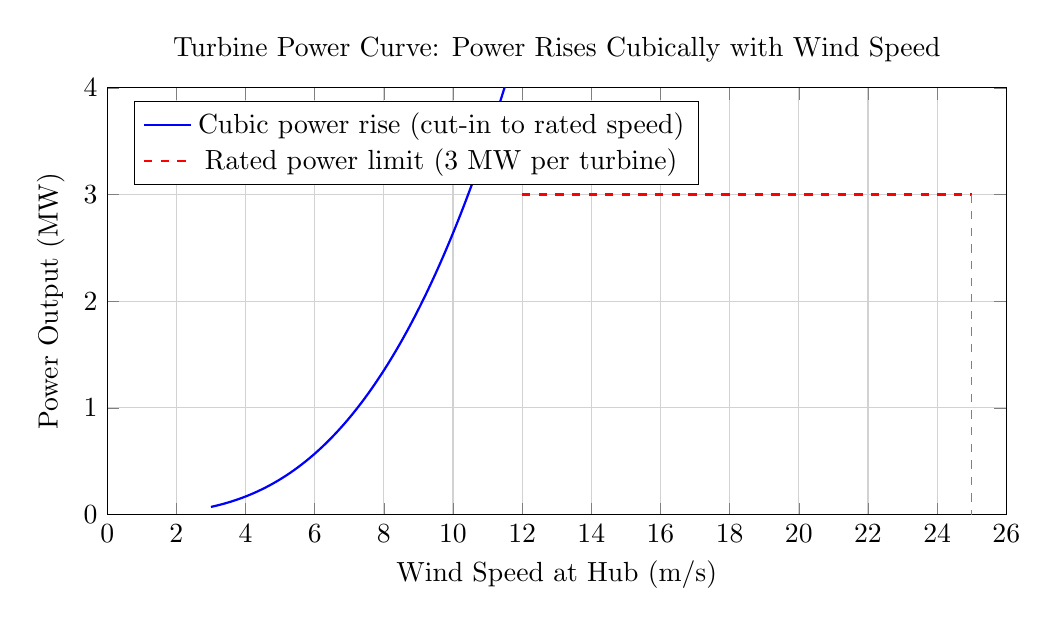
\begin{tikzpicture}
        \begin{axis}[
            xlabel={Wind Speed at Hub (m/s)},
            ylabel={Power Output (MW)},
            title={Turbine Power Curve: Power Rises Cubically with Wind Speed},
            xmin=0, xmax=26, ymin=0, ymax=4,
            grid=both,
            minor grid style={gray!15},
            major grid style={gray!35},
            width=13cm, height=7cm,
            legend pos=north west
        ]
        \addplot[blue, thick, domain=3:12, samples=80]
            {0.5 * 0.45 * 1.19 * 9852 * x^3 / 1e6};
        \addplot[red, thick, dashed]
            coordinates {(12,3.0)(25,3.0)};
        \addplot[gray, dashed]
            coordinates {(25,3.0)(25,0)};
        \addlegendentry{Cubic power rise (cut-in to rated speed)}
        \addlegendentry{Rated power limit (3 MW per turbine)}
        \end{axis}
    \end{tikzpicture}
    \caption{The turbine power curve. Power rises steeply and cubically from the cut-in wind speed until the turbine hits its rated limit, after which it is capped. Small wind speed forecast errors in the steep region cause large power errors.}
\end{figure}

\section{Generator Efficiency}

After aerodynamic power is calculated, the Physics Engine applies a small efficiency correction. At low wind speeds (below 6 m/s), a larger fraction of the generated electricity is consumed internally by the turbine's induction generator to maintain its magnetic field. This quietly reduces delivered output by an extra 1.5--3\% compared to the raw calculation.

% -----------------------------------------
\chapter{Future Work and Planned Phases}

This chapter describes the technical work currently in progress and planned for the final thesis submission.

\section{XGBoost Residual Model Training}

\subsection{The Core Idea}

The Physics Engine gives a good first estimate of power output, but it cannot model every real-world imperfection --- maintenance downtime, sensor drift, grid curtailment orders, or local turbulence patterns not captured in the weather forecast. The gap between what physics predicts and what actually comes out of the plant is called the \textbf{residual error}.

The XGBoost model is being trained to predict this error before it happens. If the model can say ``the physics estimate for the next block is likely to be 3 MW too low'', the final schedule can be adjusted upward by 3 MW before submission to CERC, keeping it within the 10\% safe zone.

\subsection{How it is Trained}

The model learns from historical SRPC data:
\begin{itemize}
    \item \textbf{Input:} The features listed in the Data Engineering chapter (time, schedule values, lagged errors).
    \item \textbf{Target:} The actual observed error for each 15-minute block (actual generation minus physics estimate).
    \item \textbf{Split:} First 8 months of data for training, last 2 months kept completely hidden for testing.
\end{itemize}

Key rule: the model is \textbf{never} asked to predict total power from scratch. It is only allowed to correct the physics estimate by predicting the error. This means the final output always respects the physical limits of the turbine (it cannot predict more power than the Betz Limit allows).

\subsection{Final Forecast Formula}

\begin{equation}
    \text{Final Schedule} = \text{Physics Estimate} + \text{XGBoost Predicted Error}
\end{equation}

The result is clipped to the valid range of 0 to 75 MW (the plant cannot produce negative power or more than its maximum capacity).

\section{Probabilistic Forecasting (Confidence Intervals)}

\subsection{Why a Single Number is Not Enough}

The current system produces one number per block: the single most likely generation value. However, wind is inherently uncertain. A plant operator submitting a schedule needs more information:

\begin{itemize}
    \item \textbf{P10 (Safe/Conservative):} A lower estimate that the plant will almost certainly exceed. Useful if the operator wants to avoid under-production penalties at all cost.
    \item \textbf{P50 (Best Estimate):} The most likely value. Balanced approach.
    \item \textbf{P90 (Optimistic):} A higher estimate. Maximises declared revenue but risks over-declaration penalties.
\end{itemize}

\subsection{Implementation Plan}

XGBoost will be retrained three times with different loss functions, each targeting a different confidence level. The plant operator can then choose which confidence band to submit based on the current electricity price and their risk tolerance for that day.

\section{Ablation Study: Separating Physics vs.\ ML Value}

A structured comparison will be run to measure how much each component of the pipeline contributes to the final accuracy improvement:

\begin{table}[H]
    \centering
    \caption{Planned Ablation Study}
    \begin{tabular}{clc}
        \toprule
        \textbf{Model} & \textbf{What is used} & \textbf{Expected error (MAE)} \\
        \midrule
        M0 & Existing grid schedule only (no changes) & 5.96 MW (Baseline) \\
        M1 & Physics Engine only (no ML correction) & To be measured \\
        M2 & XGBoost only (no physics layer) & To be measured \\
        M3 & Full PI-PML system (Physics + XGBoost) & To be measured \\
        \bottomrule
    \end{tabular}
\end{table}

This comparison will show clearly whether the improvement comes from the physics, the machine learning, or the combination.

\section{Bayesian Hyperparameter Tuning}

Standard model tuning tries to minimise prediction error in generic statistical terms. This project will go further by tuning the model to minimise the \textbf{actual financial penalty (Rs.)} incurred under CERC DSM rules. This means the tuning algorithm will learn that an error of 5 MW at 8 PM (peak pricing, 2.5$\times$ ACP multiplier) is far more costly than the same 5 MW error at 2 AM, and will adjust its parameters accordingly.

% -----------------------------------------
\chapter{Final Planned Deliverables}

The following outputs will be produced in the final phase of the thesis:

\begin{enumerate}[leftmargin=*, label=\textbf{\Alph*.}]
    \item \textbf{Accuracy Results:}
    \begin{itemize}
        \item Final comparison of schedule error (MAE) before and after the PI-PML model.
        \item Separate analysis of model performance during the July 2025 monsoon (the most volatile and financially risky period).
        \item Plots showing Actual vs.\ Predicted generation for representative weeks.
    \end{itemize}

    \item \textbf{Financial Impact Report:}
    \begin{itemize}
        \item Full simulation of CERC DSM penalties using real data, comparing the original schedule against the PI-PML corrected schedule.
        \item Quantified Rs.\ savings per month and projected annual savings.
    \end{itemize}

    \item \textbf{Scalability Discussion:}
    \begin{itemize}
        \item Assessment of how the pipeline can be adapted to other Indian wind clusters (Jaisalmer in Rajasthan, Muppandal in Tamil Nadu).
        \item Clean, well-documented Python codebase with all pipeline scripts, model files, and the financial simulator ready for demonstration.
    \end{itemize}
\end{enumerate}

% -----------------------------------------
\chapter{Conclusion}

\section{Summary of Completed Work}

This Progress Report documents the successful completion of the first phase of the PI-PML thesis project. All research and data engineering foundations are in place. Specifically:

\begin{enumerate}
    \item \textbf{CERC DSM Research:} Fully understood and documented the regulatory framework including the 4-band penalty structure and the evening peak pricing multiplier.
    \item \textbf{Site Case Study:} RSOPL Koppal (75 MW, 15.34\textdegree N 76.15\textdegree E, Vestas turbines) fully documented as the research test case.
    \item \textbf{Financial Audit:} Confirmed Rs.\ 41.34 Crores in under-production penalties from 10 months of official SRPC data --- this is the baseline the model must beat.
    \item \textbf{Data Pipeline:} 29,568 fifteen-minute blocks from 45 SRPC archives successfully cleaned, merged, and prepared as XGBoost training labels.
    \item \textbf{NWP Evaluation:} Three weather data systems compared. NOAA GFS selected for live inference; BFS planned as future upgrade.
    \item \textbf{Physics Engine:} Fully implemented in Python --- takes weather forecast data in, produces accurate theoretical power estimates out, with moist air density correction and Hellman height adjustment applied.
\end{enumerate}

\section{Outlook}

With the data foundation and physics baseline complete, the project is well-positioned to deliver the machine learning training, financial validation, and probabilistic forecasting components on schedule. The core technical architecture is sound, the data is clean, and the financial impact opportunity is clearly defined and quantified.

% -----------------------------------------
\begin{thebibliography}{9}

\bibitem{cerc2024}
Central Electricity Regulatory Commission (CERC),
\textit{Deviation Settlement Mechanism and Related Matters Regulations, 2024}.
Available: \url{https://www.cercind.gov.in}

\bibitem{srpc2025}
Southern Regional Power Committee (SRPC),
\textit{Public Commercial DSM Accounts --- RSOPL Koppal, 2025--26}.
Available: \url{https://srpc.kar.nic.in}

\bibitem{chen2016}
T. Chen and C. Guestrin,
``XGBoost: A Scalable Tree Boosting System,''
\textit{Proc.\ 22nd ACM SIGKDD}, pp.\ 785--794, 2016.

\bibitem{karpatne2017}
A. Karpatne et al.,
``Theory-Guided Data Science: A New Paradigm for Scientific Discovery,''
\textit{IEEE Trans.\ Knowl.\ Data Eng.}, vol.\ 29, no.\ 10, pp.\ 2318--2331, 2017.

\bibitem{windpowerlib}
windpowerlib Development Team,
\textit{windpowerlib: A Python library for wind turbine modelling}, 2023.
Available: \url{https://windpowerlib.readthedocs.io}

\bibitem{iex2024}
Indian Energy Exchange (IEX),
\textit{Area Clearing Price Market Reports, 2024--25}.
Available: \url{https://www.iexindia.com}

\end{thebibliography}

\end{document}
